\documentclass{beamer}\usepackage[]{graphicx}\usepackage[]{color}
%% maxwidth is the original width if it is less than linewidth
%% otherwise use linewidth (to make sure the graphics do not exceed the margin)
\makeatletter
\def\maxwidth{ %
  \ifdim\Gin@nat@width>\linewidth
    \linewidth
  \else
    \Gin@nat@width
  \fi
}
\makeatother

\definecolor{fgcolor}{rgb}{0.345, 0.345, 0.345}
\newcommand{\hlnum}[1]{\textcolor[rgb]{0.686,0.059,0.569}{#1}}%
\newcommand{\hlstr}[1]{\textcolor[rgb]{0.192,0.494,0.8}{#1}}%
\newcommand{\hlcom}[1]{\textcolor[rgb]{0.678,0.584,0.686}{\textit{#1}}}%
\newcommand{\hlopt}[1]{\textcolor[rgb]{0,0,0}{#1}}%
\newcommand{\hlstd}[1]{\textcolor[rgb]{0.345,0.345,0.345}{#1}}%
\newcommand{\hlkwa}[1]{\textcolor[rgb]{0.161,0.373,0.58}{\textbf{#1}}}%
\newcommand{\hlkwb}[1]{\textcolor[rgb]{0.69,0.353,0.396}{#1}}%
\newcommand{\hlkwc}[1]{\textcolor[rgb]{0.333,0.667,0.333}{#1}}%
\newcommand{\hlkwd}[1]{\textcolor[rgb]{0.737,0.353,0.396}{\textbf{#1}}}%

\usepackage{framed}
\makeatletter
\newenvironment{kframe}{%
 \def\at@end@of@kframe{}%
 \ifinner\ifhmode%
  \def\at@end@of@kframe{\end{minipage}}%
  \begin{minipage}{\columnwidth}%
 \fi\fi%
 \def\FrameCommand##1{\hskip\@totalleftmargin \hskip-\fboxsep
 \colorbox{shadecolor}{##1}\hskip-\fboxsep
     % There is no \\@totalrightmargin, so:
     \hskip-\linewidth \hskip-\@totalleftmargin \hskip\columnwidth}%
 \MakeFramed {\advance\hsize-\width
   \@totalleftmargin\z@ \linewidth\hsize
   \@setminipage}}%
 {\par\unskip\endMakeFramed%
 \at@end@of@kframe}
\makeatother

\definecolor{shadecolor}{rgb}{.97, .97, .97}
\definecolor{messagecolor}{rgb}{0, 0, 0}
\definecolor{warningcolor}{rgb}{1, 0, 1}
\definecolor{errorcolor}{rgb}{1, 0, 0}
\newenvironment{knitrout}{}{} % an empty environment to be redefined in TeX

\usepackage{alltt} 

\usepackage{graphics}
\usepackage[T1]{fontenc}
\setbeamercovered{transparent}
\renewcommand{\ni}{\noindent}

%load packages that will be invisible on slides


\title[ 1-Intro]{Day 2 - Advanced Graphics in R}
\subtitle{05 - Plotting Map Data}
\date{\hspace{1in}}
\institute[ISU]{Iowa State University}
\IfFileExists{upquote.sty}{\usepackage{upquote}}{}
\begin{document}

\begin{frame}
    \maketitle
\end{frame}


%-----------------------------------------------------------------------------

\begin{frame}[fragile]
    \frametitle{What is a Map?}

A bunch of latitude longitude points...

\small
\begin{knitrout}\footnotesize
\definecolor{shadecolor}{rgb}{1, 1, 1}\color{fgcolor}\begin{kframe}
\begin{alltt}
\hlkwd{qplot}\hlstd{(long, lat,} \hlkwc{geom}\hlstd{=}\hlstr{"point"}\hlstd{,} \hlkwc{data}\hlstd{=states)}
\end{alltt}
\end{kframe}
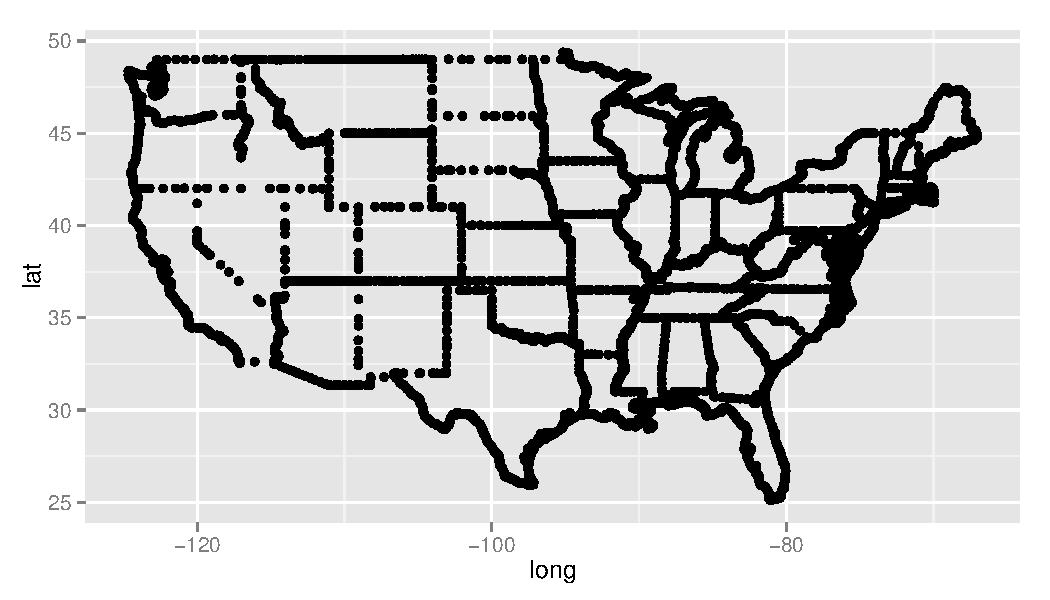
\includegraphics[width=\textwidth]{figure/kmappoints} 

\end{knitrout}
    \normalsize
\end{frame}

%-----------------------------------------------------------------------------

\begin{frame}[fragile]
    \frametitle{What is a Map?}

... that are connected with lines in a very specific order.

\small
\begin{knitrout}\footnotesize
\definecolor{shadecolor}{rgb}{1, 1, 1}\color{fgcolor}\begin{kframe}
\begin{alltt}
\hlkwd{qplot}\hlstd{(long, lat,} \hlkwc{geom}\hlstd{=}\hlstr{"path"}\hlstd{,} \hlkwc{data}\hlstd{=states,} \hlkwc{group}\hlstd{=group)} \hlopt{+} \hlkwd{coord_map}\hlstd{()}
\end{alltt}
\end{kframe}
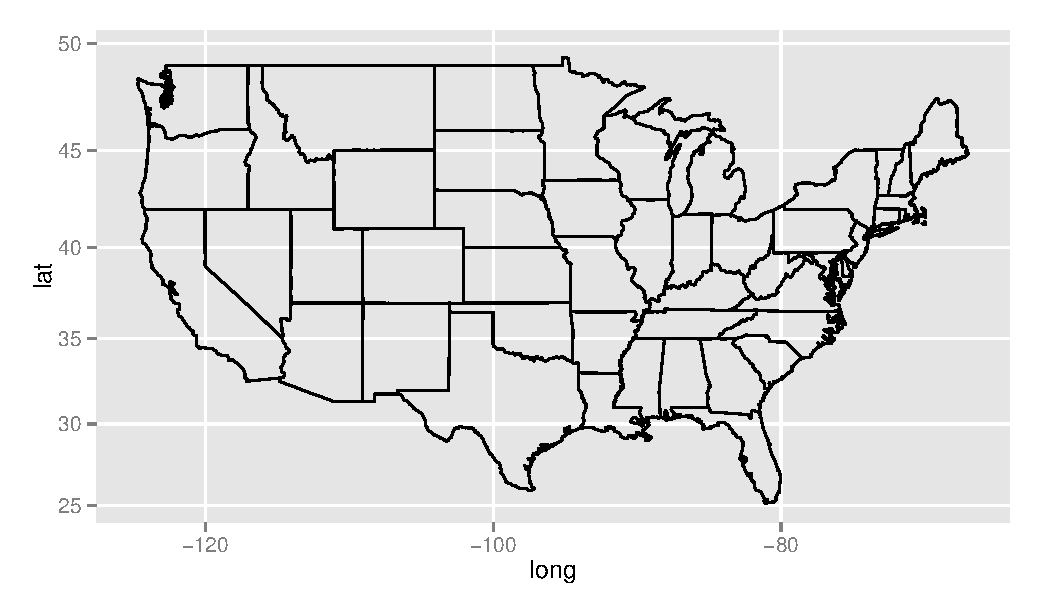
\includegraphics[width=\textwidth]{figure/kmapoutline} 

\end{knitrout}
    \normalsize
\end{frame}


%-----------------------------------------------------------------------------

\begin{frame}
    \frametitle{Basic Map Data}
  What needs to be in the data set in order to plot a basic map?
    \begin{itemize}
        \item Need latitude/longitude points for all map boundaries
        \item Need to know which boundary group all lat/long points belong
        \item Need to know the order to connect points within each group
    \end{itemize}    
\end{frame}

%-----------------------------------------------------------------------------

\begin{frame}[fragile]
    \frametitle{Data for Building Basic State Map}
    
 Our \texttt{states} data has all necessary information
    
    \small
\begin{knitrout}\footnotesize
\definecolor{shadecolor}{rgb}{1, 1, 1}\color{fgcolor}\begin{kframe}
\begin{alltt}
\hlstd{states} \hlkwb{<-} \hlkwd{map_data}\hlstd{(}\hlstr{"state"}\hlstd{)}
\hlkwd{head}\hlstd{(states)}
\end{alltt}
\begin{verbatim}
##     long   lat group order  region subregion
## 1 -87.46 30.39     1     1 alabama      <NA>
## 2 -87.48 30.37     1     2 alabama      <NA>
## 3 -87.53 30.37     1     3 alabama      <NA>
## 4 -87.53 30.33     1     4 alabama      <NA>
## 5 -87.57 30.33     1     5 alabama      <NA>
## 6 -87.59 30.33     1     6 alabama      <NA>
\end{verbatim}
\end{kframe}
\end{knitrout}
    \normalsize
\end{frame}


%-----------------------------------------------------------------------------

\begin{frame}
    \frametitle{Incorporating Information About States}
  Want to incorporate additional information into the plot:
    \begin{itemize}
        \item Add other geographic information by adding geometric layers to the plot
        \item Add non-geopgraphic information by altering the fill color for each state
      \begin{itemize}
        \item Use \texttt{geom=''polygon''} to treat states as solid shapes to add color
        \item Incorporate numeric information using color shade or intensity
        \item Incorporate categorical informaion using color hue
      \end{itemize}
    \end{itemize}    
\end{frame}

%-----------------------------------------------------------------------------

\begin{frame}[fragile]
    \frametitle{Categorical Information Using Hue}
If a categorical variable is assigned as the fill color then \texttt{qplot} will assign different hues for each category
    
    \small
\begin{knitrout}\footnotesize
\definecolor{shadecolor}{rgb}{1, 1, 1}\color{fgcolor}\begin{kframe}
\begin{alltt}
\hlkwd{qplot}\hlstd{(long, lat,} \hlkwc{geom}\hlstd{=}\hlstr{"polygon"}\hlstd{,} \hlkwc{data}\hlstd{=states.class.map,} \hlkwc{group}\hlstd{=group,} \hlkwc{fill}\hlstd{=StateGroups,} \hlkwc{colour}\hlstd{=}\hlkwd{I}\hlstd{(}\hlstr{"black"}\hlstd{))} \hlopt{+} \hlkwd{coord_map}\hlstd{()}
\end{alltt}
\end{kframe}
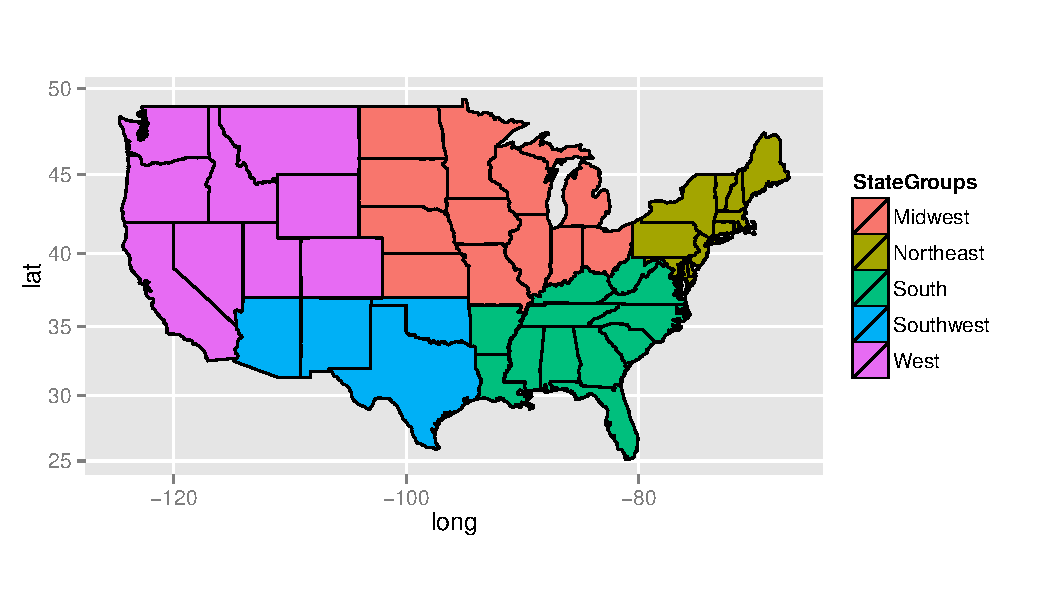
\includegraphics[width=\textwidth]{figure/kstatescolored} 

\end{knitrout}
    \normalsize
\end{frame}

%-----------------------------------------------------------------------------

\begin{frame}
    \frametitle{Numerical Information Using Shade and Intensity}
    
    To show how was can add numerical information to map plots we will use the BRFSS data
    
    \begin{itemize}
        \item Behavioral Risk Factor Surveillance System
        \item 2008 telephone survey run by the Center for Disease Control (CDC)
        \item Ask a variety of questions related to health and wellness
        \item Cleaned data with state aggregated values posted on website
    \end{itemize}    
\end{frame}


%-----------------------------------------------------------------------------

\begin{frame}[fragile]
    \frametitle{BRFSS Data Aggregated by State}
    
    
    \small
\begin{knitrout}\footnotesize
\definecolor{shadecolor}{rgb}{1, 1, 1}\color{fgcolor}\begin{kframe}
\begin{alltt}
\hlkwd{head}\hlstd{(states.stats)}
\end{alltt}
\begin{verbatim}
##   state.name avg.wt avg.qlrest2 avg.ht avg.bmi avg.drnk
## 1    alabama  180.7       9.051  168.0   29.00    2.333
## 2     alaska  189.3       8.381  172.1   28.91    2.324
## 3    arizona  169.7       5.770  168.3   27.05    2.407
## 4   arkansas  177.4       8.227  168.8   28.02    2.312
## 5 california  170.0       6.848  168.1   27.23    2.170
## 6   colorado  167.2       8.135  169.6   26.17    1.971
\end{verbatim}
\end{kframe}
\end{knitrout}
    \normalsize
\end{frame}

%-----------------------------------------------------------------------------

\begin{frame}[fragile]
    \frametitle{Numerical Information Using Shade and Intensity}

Average number of days in the last 30 days of insufficient sleep by state

\small
\begin{knitrout}\footnotesize
\definecolor{shadecolor}{rgb}{1, 1, 1}\color{fgcolor}\begin{kframe}
\begin{alltt}
\hlkwd{qplot}\hlstd{(long, lat,} \hlkwc{geom}\hlstd{=}\hlstr{"polygon"}\hlstd{,} \hlkwc{data}\hlstd{=states.map,} \hlkwc{group}\hlstd{=group,} \hlkwc{fill}\hlstd{=avg.qlrest2)} \hlopt{+} \hlkwd{coord_map}\hlstd{()}
\end{alltt}
\end{kframe}
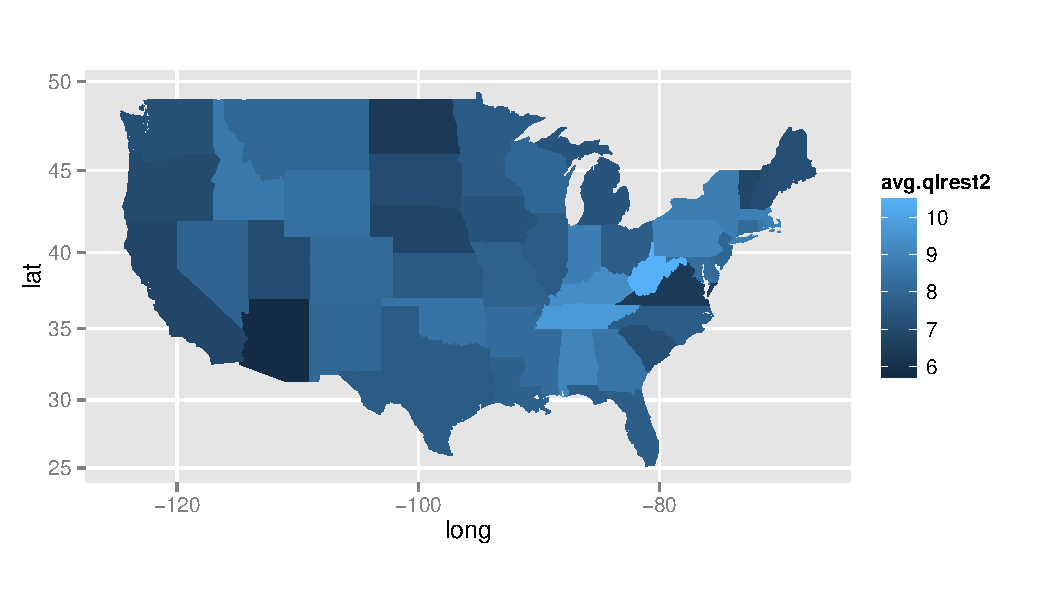
\includegraphics[width=\textwidth]{figure/ksleepdep} 

\end{knitrout}
    \normalsize
\end{frame}


%-----------------------------------------------------------------------------

\begin{frame}[fragile]
    \frametitle{BRFSS Data Aggregated by State and Gender}
    
    \small
\begin{knitrout}\footnotesize
\definecolor{shadecolor}{rgb}{1, 1, 1}\color{fgcolor}\begin{kframe}
\begin{alltt}
\hlkwd{head}\hlstd{(states.sex.stats)}
\end{alltt}
\begin{verbatim}
##   state.name SEX avg.wt avg.qlrest2 avg.ht avg.bmi avg.drnk    sex
## 1    alabama   1  198.9       8.649  177.6   28.51    3.033   Male
## 2    alabama   2  173.0       9.225  164.0   29.21    2.042 Female
## 3     alaska   1  203.4       7.236  178.4   28.91    2.487   Male
## 4     alaska   2  169.6       9.907  163.1   28.89    2.103 Female
## 5    arizona   1  191.4       5.164  177.2   27.63    2.814   Male
## 6    arizona   2  156.2       6.143  162.7   26.68    2.027 Female
\end{verbatim}
\end{kframe}
\end{knitrout}
    \normalsize
\end{frame}


%-----------------------------------------------------------------------------

\begin{frame}[fragile]
    \frametitle{Adding Numerical Information}

Average number of alcoholic drinks per day by state and gender

\begin{knitrout}\footnotesize
\definecolor{shadecolor}{rgb}{1, 1, 1}\color{fgcolor}\begin{kframe}
\begin{alltt}
\hlkwd{qplot}\hlstd{(long, lat,} \hlkwc{geom}\hlstd{=}\hlstr{"polygon"}\hlstd{,} \hlkwc{data}\hlstd{=states.sex.map,} \hlkwc{group}\hlstd{=group,} \hlkwc{fill}\hlstd{=avg.drnk)} \hlopt{+}  \hlkwd{coord_map}\hlstd{()} \hlopt{+} \hlkwd{facet_grid}\hlstd{(sex} \hlopt{~} \hlstd{.)}
\end{alltt}
\end{kframe}
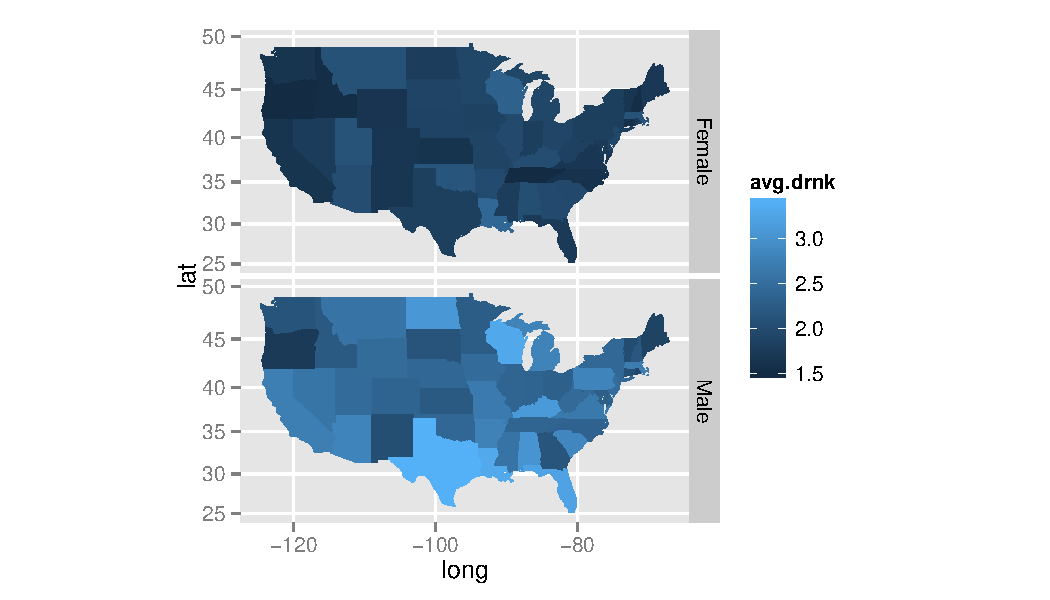
\includegraphics[width=\textwidth]{figure/kalcohol1} 

\end{knitrout}
\end{frame}

%-----------------------------------------------------------------------------

\begin{frame}
    \frametitle{Your Turn}
    Use \texttt{merge} to combine child healthcare data with maps information \\
    
    \vspace{.4in}
    
    Then use \texttt{qplot} to create a map of child healthcare undercoverage rate by state
 
\end{frame}

%-----------------------------------------------------------------------------

\begin{frame}
    \frametitle{Cleaning Up Your Maps}
   Use ggplot2 options to clean up your map!
    \begin{itemize}
      \item Adding Titles \texttt{ + ggtitle(...)}
      \item Might want a plain white background \texttt{ + theme\_bw()}
      \item Extremely familiar geography may eliminate need for latitude and longitude axes \texttt{ + theme(...)}
      \item Want to customize color gradient   \texttt{ + scale\_fill\_gradient2(...) }
      \item Keep aspect ratios correct   \texttt{ + coord\_map() }
    \end{itemize}    
\end{frame}



%-----------------------------------------------------------------------------

\begin{frame}[fragile]
    \frametitle{Cleaning Up Your Maps}

\begin{knitrout}\footnotesize
\definecolor{shadecolor}{rgb}{1, 1, 1}\color{fgcolor}\begin{kframe}
\begin{alltt}
\hlkwd{qplot}\hlstd{(long, lat,} \hlkwc{geom}\hlstd{=}\hlstr{"polygon"}\hlstd{,} \hlkwc{data}\hlstd{=states.map,} \hlkwc{group}\hlstd{=group,} \hlkwc{fill}\hlstd{=avg.drnk)} \hlopt{+}
  \hlkwd{coord_map}\hlstd{()} \hlopt{+}  \hlkwd{theme_bw}\hlstd{()} \hlopt{+}
  \hlkwd{scale_fill_gradient2}\hlstd{(}\hlkwc{limits}\hlstd{=}\hlkwd{c}\hlstd{(}\hlnum{1.5}\hlstd{,} \hlnum{3}\hlstd{),}\hlkwc{low}\hlstd{=}\hlstr{"lightgray"}\hlstd{,}\hlkwc{high}\hlstd{=}\hlstr{"red"}\hlstd{)} \hlopt{+}
  \hlkwd{theme}\hlstd{(}\hlkwc{axis.ticks} \hlstd{=} \hlkwd{element_blank}\hlstd{(),}
       \hlkwc{axis.text.x} \hlstd{=} \hlkwd{element_blank}\hlstd{(),}
       \hlkwc{axis.title.x}\hlstd{=}\hlkwd{element_blank}\hlstd{(),}
       \hlkwc{axis.text.y} \hlstd{=} \hlkwd{element_blank}\hlstd{(),}
       \hlkwc{axis.title.y}\hlstd{=}\hlkwd{element_blank}\hlstd{())} \hlopt{+}
  \hlkwd{ggtitle}\hlstd{(}\hlstr{"Map of Average Number of Alcoholic Beverages Consumed Per Day by State"}\hlstd{)}
\end{alltt}
\end{kframe}
\end{knitrout}
\end{frame}
 
%-----------------------------------------------------------------------------

\begin{frame}[fragile]
    \frametitle{Cleaning Up Your Maps}

\begin{knitrout}\footnotesize
\definecolor{shadecolor}{rgb}{1, 1, 1}\color{fgcolor}
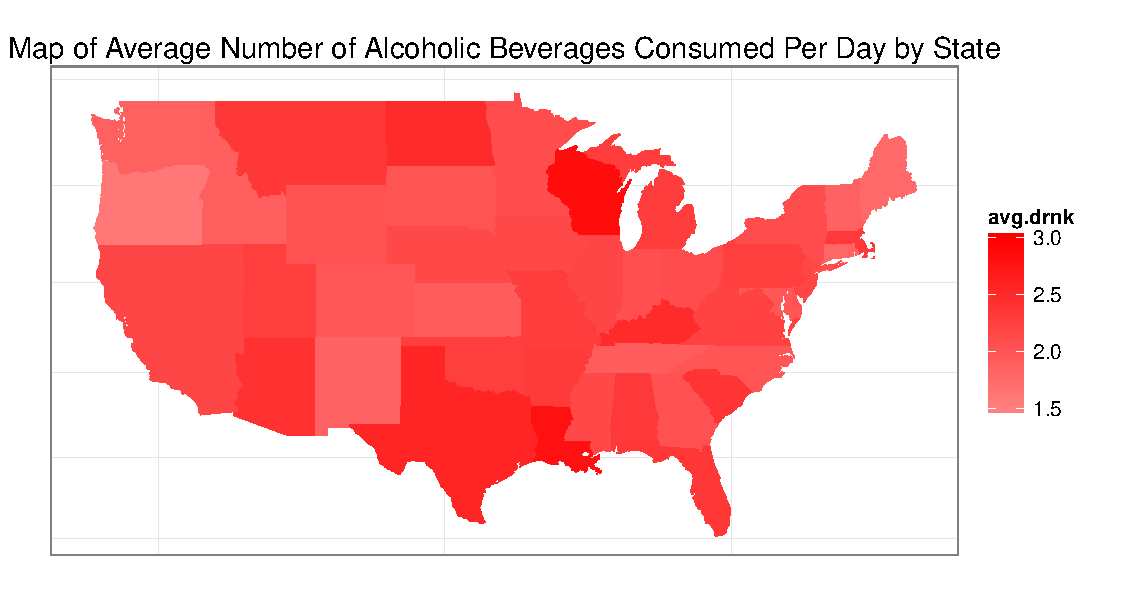
\includegraphics[width=\textwidth]{figure/kalcohol3} 

\end{knitrout}
\end{frame}


%-----------------------------------------------------------------------------

\begin{frame}[fragile]
    \frametitle{Cleaning Up Your Maps}

\begin{knitrout}\footnotesize
\definecolor{shadecolor}{rgb}{1, 1, 1}\color{fgcolor}\begin{kframe}
\begin{alltt}
\hlkwd{qplot}\hlstd{(long, lat,} \hlkwc{geom}\hlstd{=}\hlstr{"polygon"}\hlstd{,} \hlkwc{data}\hlstd{=states.sex.map,} \hlkwc{group}\hlstd{=group,} \hlkwc{fill}\hlstd{=avg.drnk)} \hlopt{+}
  \hlkwd{coord_map}\hlstd{()} \hlopt{+} \hlkwd{facet_grid}\hlstd{(sex} \hlopt{~} \hlstd{.)} \hlopt{+}
  \hlkwd{theme_bw}\hlstd{()} \hlopt{+}
  \hlkwd{scale_fill_gradient2}\hlstd{(}\hlkwc{limits}\hlstd{=}\hlkwd{c}\hlstd{(}\hlnum{1.5}\hlstd{,} \hlnum{4}\hlstd{),}\hlkwc{low}\hlstd{=}\hlstr{"lightgray"}\hlstd{,}\hlkwc{high}\hlstd{=}\hlstr{"red"}\hlstd{)} \hlopt{+}
  \hlkwd{theme}\hlstd{(}\hlkwc{axis.ticks} \hlstd{=} \hlkwd{element_blank}\hlstd{(),}
       \hlkwc{axis.text.x} \hlstd{=} \hlkwd{element_blank}\hlstd{(),}
       \hlkwc{axis.title.x}\hlstd{=}\hlkwd{element_blank}\hlstd{(),}
       \hlkwc{axis.text.y} \hlstd{=} \hlkwd{element_blank}\hlstd{(),}
       \hlkwc{axis.title.y}\hlstd{=}\hlkwd{element_blank}\hlstd{())} \hlopt{+}
  \hlkwd{ggtitle}\hlstd{(}\hlstr{"Map of Average Number of Alcoholic Beverages Consumed Per Day by State and Gender"}\hlstd{)}
\end{alltt}
\end{kframe}
\end{knitrout}
\end{frame}
 
%-----------------------------------------------------------------------------

\begin{frame}[fragile]
    \frametitle{Cleaning Up Your Maps}

\begin{knitrout}\footnotesize
\definecolor{shadecolor}{rgb}{1, 1, 1}\color{fgcolor}
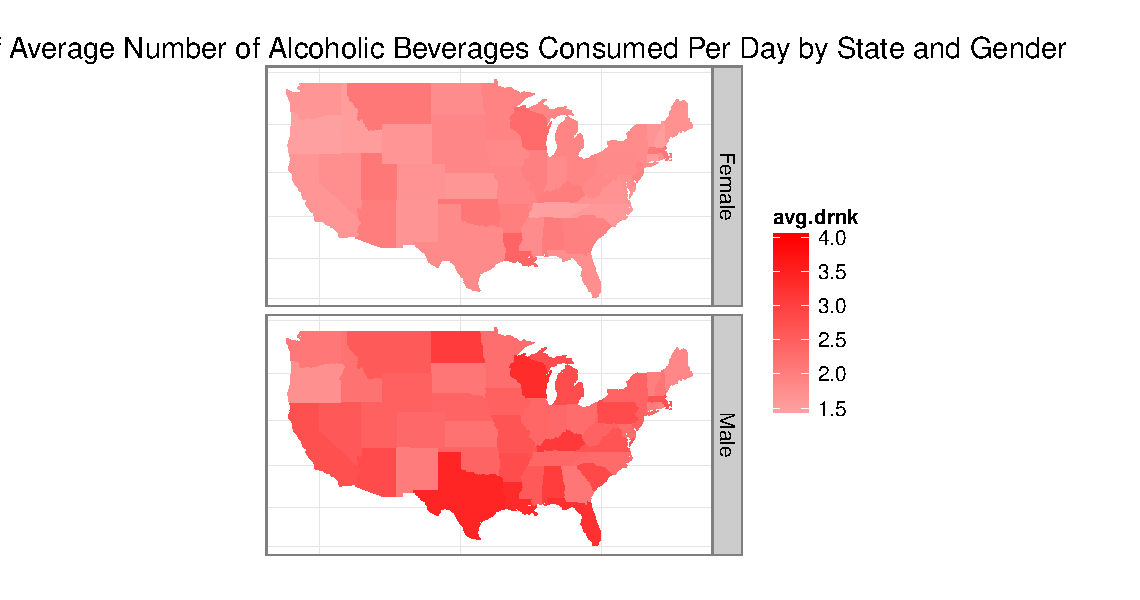
\includegraphics[width=\textwidth]{figure/kalcohol5} 

\end{knitrout}
\end{frame}


%-----------------------------------------------------------------------------

\begin{frame}
    \frametitle{Your Turn}
    Use options to polish the look of your map of child healthcare undercoverage rate by state!
    
\end{frame}

\end{document}
